\documentclass{beamer}
\usepackage[UTF8]{ctex}
\usepackage{amsmath,amsfonts,amssymb,bm}
\usepackage{graphicx}
\usepackage{hyperref}

\title{基于标签分布感知间隔损失的\\不平衡数据学习}
\subtitle{Learning Imbalanced Datasets with Label-Distribution-Aware Margin Loss}
\author{报告人:乔彦博}
\institute{LDAM损失函数margin的推导证明}
\date{\today}

\begin{document}

\begin{frame}
    \titlepage
\end{frame}

\begin{frame}
    \centering {\LARGE 内容提要}
\vspace{1em}
\begin{flushleft}
    \tableofcontents
\end{flushleft}
\end{frame}

\section{数据不平衡学习背景}
\begin{frame}{长尾分布问题}
    % 此处建议插入图:长尾分布示意图(类别频次的长尾分布曲线)
    \begin{figure}[h]
        \centering
        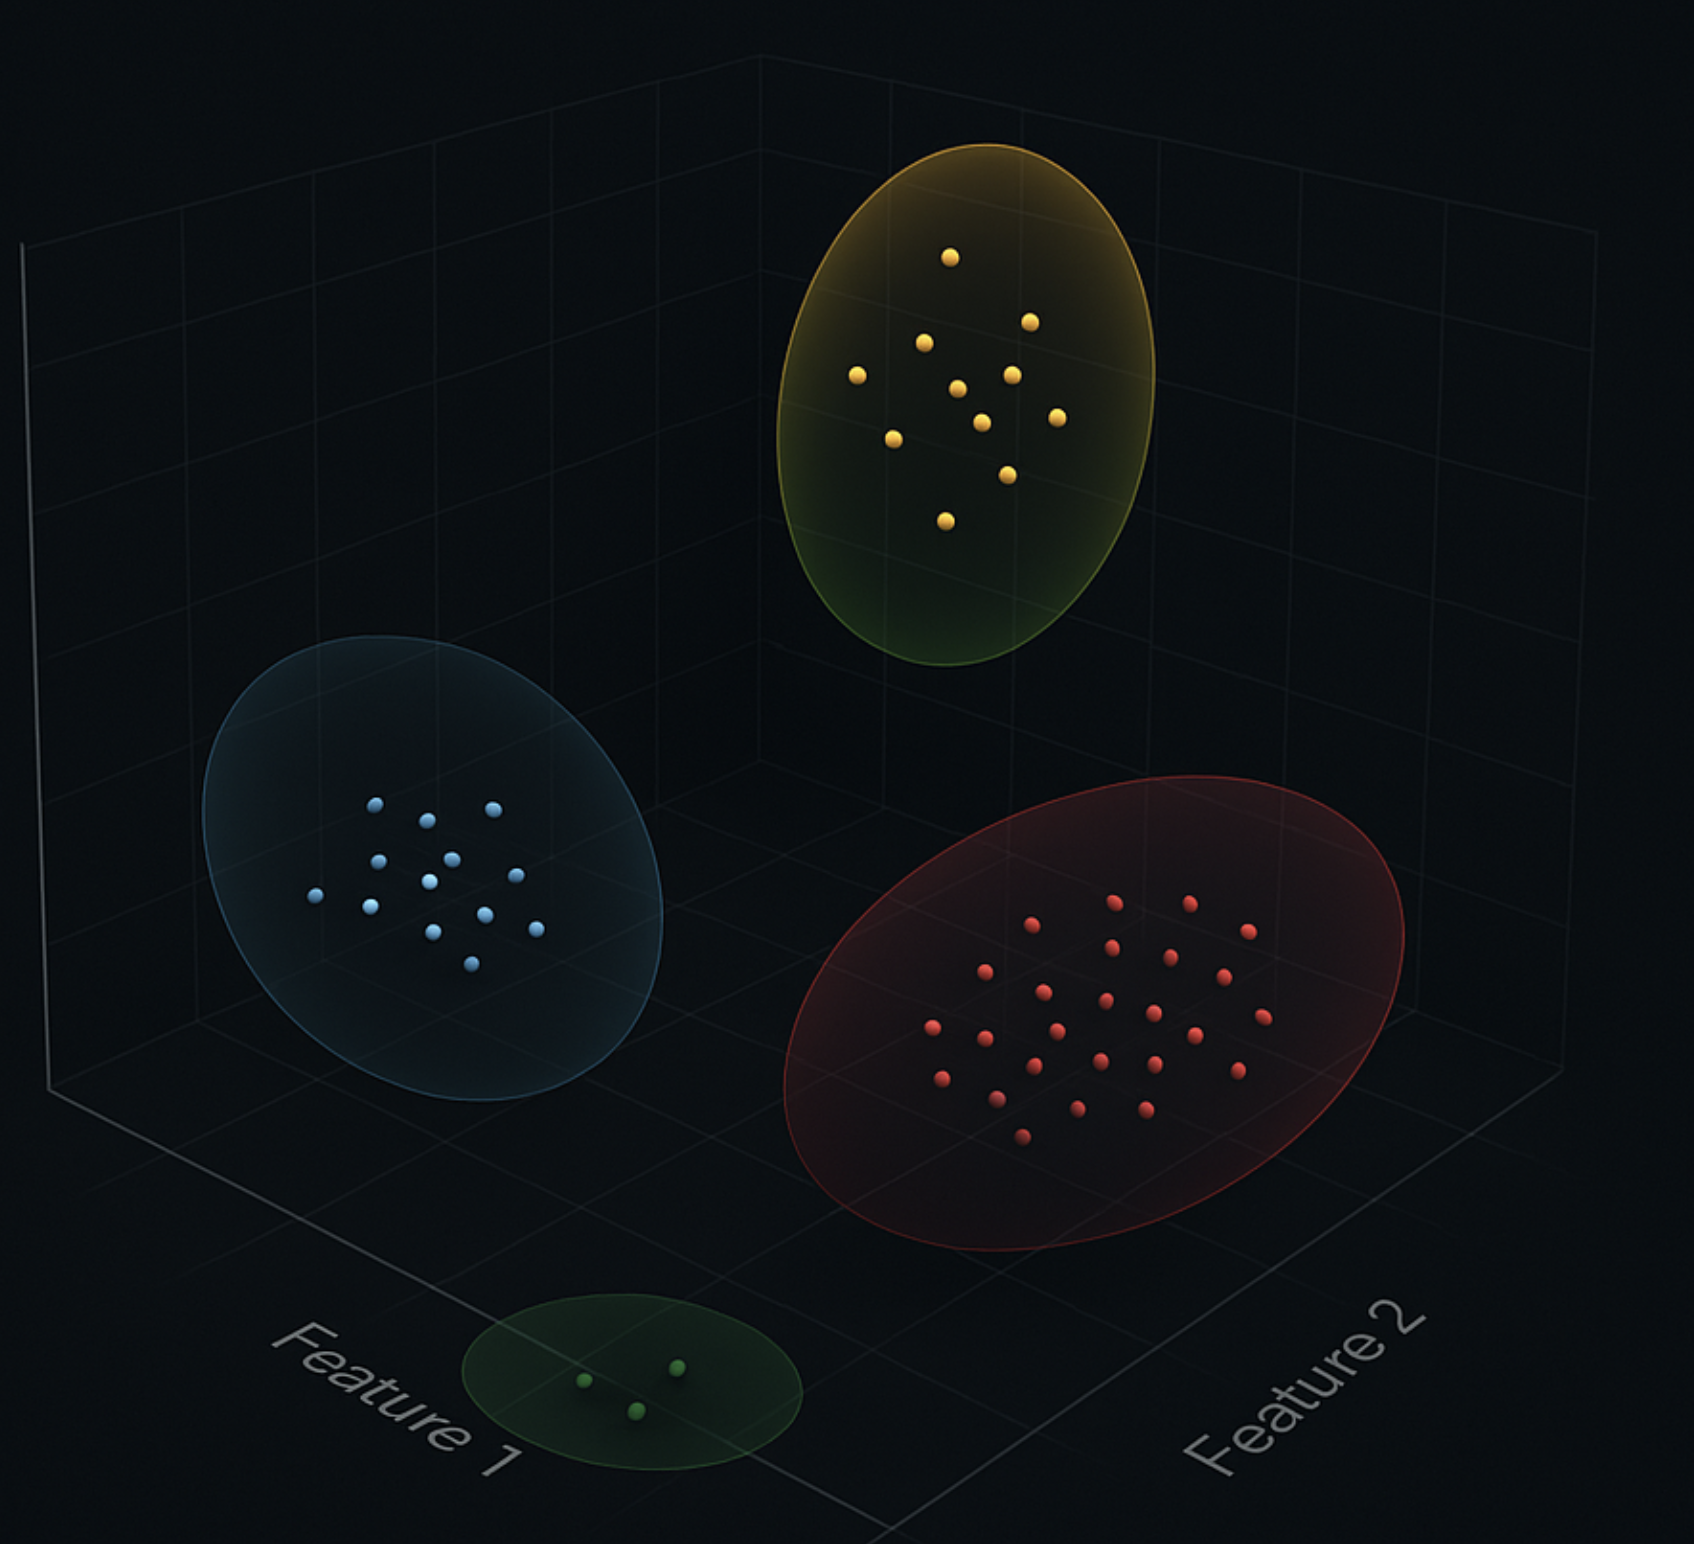
\includegraphics[width=0.7\linewidth]{long-tail.png}
        \caption{长尾分布示意图}
    \end{figure}
\end{frame}
\begin{frame}{长尾分布的训练难题}
    \begin{itemize}
        \item \textbf{头部挤占空间和边界}:在长尾分布下,头部类别(样本多)在特征空间中占据主导地位,导致尾部类别(样本少)可用的判别空间被严重压缩,决策边界容易偏向头部类。
        \item \textbf{尾部样本少,难以支撑空间和间隔}:尾部类别由于样本极少,模型难以学习到稳定且具有代表性的特征,导致其决策边界不明确,分类间隔(margin)很小,泛化能力差,易被头部类误分类。
        \item 这两大难题共同导致尾部类别的准确率显著低于头部类别,是长尾分布下模型训练的核心挑战。
    \end{itemize}
\end{frame}

\begin{frame}{常规应对方法}
    \begin{itemize}
        \item \textbf{重采样(Re-sampling)}:对多数类\textbf{欠采样}或对少数类\textbf{过采样},使训练集类分布平衡。但过采样易造成少数类\textbf{过拟合},欠采样会丢失多数类信息。
        \item \textbf{重加权(Re-weighting)}:在损失函数中给予少数类样本更大权重。例如按照类别频数的倒数加权。但权重过大时训练不稳定,容易\textbf{优化困难}。
        \item 其他方法:如\textbf{特殊损失函数}(Focal Loss 等)降低易分类样本权重,或\textbf{两阶段训练}(先学特征再调分类器)等。
        \item 常规方法局限:重采样/重加权在深度网络中效果不稳(易过拟合或需精调超参),有动机探索新的不平衡学习策略。
    \end{itemize}
\end{frame}

\section{LDAM 的动机与核心思想}
\begin{frame}{LDAM 的动机与核心思想}
    \begin{itemize}
        \item \textbf{核心动机}: 少数类样本少,易过拟合,泛化误差高,需要更大的分类间隔(margin)提升鲁棒性。
        \item \textbf{关键思想}: 分类间隔应依赖类别标签,样本越少的类别,间隔应越大。
        \item \textbf{LDAM方法}: 在损失函数中引入类别相关的间隔偏移
        \[
            \Delta_j = C \cdot n_j^{-1/4}
        \]
        少数类判别要求更高置信度,提升平衡准确率。
    \end{itemize}
\end{frame}

\section{LDAM 损失函数形式}
\begin{frame}{LDAM 损失函数(Hinge 形式)}
    考虑模型对样本 $(x,y)$ 输出各类别的实数分数(logits)$z_1, z_2, \dots, z_k$。为简化记号,记 $z_j = f(x)_j$。
    \begin{itemize}
        \item \textbf{间隔损失(多分类 Hinge 扩展)}: 
        \[
            L_{\text{LDAM-HG}}(x,y) = \max\{\max_{j \neq y}(z_j) - z_y + \Delta_y,\;0\}\,,
        \] 
        其中 $\Delta_y$ 为类别 $y$ 的间隔偏移量(下同)。
        \item 含义:要求正确类得分 $z_y$ 比任何错误类得分至少高出 $\Delta_y$。若差值小于 $\Delta_y$ 则产生损失,促使模型拉大该差距。
        \item 间隔偏移设定为 $\displaystyle \Delta_j = C \cdot n_j^{-1/4}$,其中 $C$ 为超参数。少数类因 $n_j$ 小而 $\Delta_j$ 大,需要更大间隔方可零损失。
        \item Hinge 损失不连续,直接优化可能有困难。
    \end{itemize}
\end{frame}

\begin{frame}{LDAM 损失函数(交叉熵形式)}
    \begin{itemize}
        \item \textbf{平滑的交叉熵损失}: 为了优化的稳定性,LDAM 实际采用交叉熵形式加入间隔:
        \[
            L_{\text{LDAM}}(x,y) = -\log \frac{\exp(z_y - \Delta_y)}{\exp(z_y - \Delta_y) + \sum_{j \neq y}\exp(z_j)}\,,
        \] 
        其中同样 $\Delta_y = C \cdot n_y^{-1/4}$。
        \item 对正确类别的 logit 减去 $\Delta_y$,相当于提高该样本被正确分类的难度(需要更大的 logit 才有相同概率),从而有效地在概率空间实现了类依赖的间隔。
        \item 当训练集平衡时,可以视 $\Delta_y$ 取常数 $C$(不区分类别)即退化为一般的具有固定 margin 的损失【与以往工作中恒定 margin 的情况对应】。LDAM 则针对不平衡数据,动态调整 margin 大小。
        \item 总体而言,LDAM 通过简单修改损失函数,结合后续的训练策略(如延迟重加权),取得了优于单纯重采样/重加权的方法的效果。
    \end{itemize}
\end{frame}

\section{定理一推导}
\begin{frame}{平衡误差与分类间隔}
    \begin{itemize}
        \item 考虑\textbf{平衡测试误差}:各类测试样本数均等时,模型的总体误分类率记为 $L_{\text{bal}}$。若 $L_j$ 表示类别 $j$ 上的误差率(即真实标签为 $j$ 时的错误率),则 
        \[
            L_{\text{bal}} = \frac{1}{k}\sum_{j=1}^k L_j\,,
        \] 
        即各类误差的平均。
        \item \textbf{分类间隔(margin)}: 对于类别 $j$,可以定义模型的\textbf{训练间隔} $\gamma_j$ 为该类训练样本距决策边界的最小距离(几何间隔),或等价地在多分类情形下定义为 $\gamma_j = \min_{x_i:y_i=j}\big(f(x_i)_y - \max_{l \neq y}f(x_i)_l\big)$。$\gamma_j$ 越大表示类别 $j$ 的训练样本与其他类别分得越开。
        \item 理论上,较大的 $\gamma_j$ 有助于降低类别 $j$ 的泛化误差。我们将利用\textbf{基于间隔的泛化界}来分析不平衡数据下的误差。
    \end{itemize}
\end{frame}

\begin{frame}{整体间隔界(标签无关)}
    在传统均衡情形,有如下经典结果:若模型对所有训练样本都实现了至少 $\gamma$ 的间隔,则测试误差有上界(以高概率):
    \[
        L_{\text{test}} \lesssim \frac{C(F)}{\gamma^2\,n}\,,
    \] 
    其中 $n$ 是训练集大小,$C(F)$ 表示模型空间的复杂度常数(如VC维或 Rademacher 复杂度相关因子)。该上界展示了错误率随样本数增加而降低,并随间隔增大而降低。
    \begin{itemize}
        \item 然而,上式中的 $\gamma$ 取决于所有样本中的最小间隔,即主要由数据最密集的多数类限制,\textbf{没有反映类别不平衡}。
        \item 为了针对不平衡情况进行更精细的分析,我们需要考察每一类别各自的间隔和规模对误差的影响。
    \end{itemize}
\end{frame}

\begin{frame}{按类别的间隔泛化界}
    \textbf{定理1(简化表述)}: 假设模型对每个类别 $j$ 的训练样本均实现了至少 $\gamma_j$ 的间隔,则以高概率,有:
    \[
        L_j \;\lesssim\; \frac{1}{\gamma_j}\sqrt{\frac{C(F)}{\,n_j\,}} \;+\; \frac{\log n}{\sqrt{\,n_j\,}}\,,
    \] 
    其中 $n_j$ 是类别 $j$ 的训练样本数,$C(F)$为假设类的复杂度常数。符号 $\lesssim$ 表示忽略了与 $\delta$ 概率有关的次要常数项。
    \begin{itemize}
        \item 直观理解:类别 $j$ 的\textbf{泛化误差}上界随 $n_j$ 增大而降低,并随 $\gamma_j$ 增大而降低。第二项 $\frac{\log n}{\sqrt{n_j}}$ 相对第一项为低阶项(当 $n_j$ 较大时)。
        \item 因此对于样本较少($n_j$ 小)的类别,要保证同等的误差上限,需要更大的 $\gamma_j$ 才行。这正定量地说明了为什么少数类需要更大的间隔来提升泛化性能。
    \end{itemize}
\end{frame}

\begin{frame}{平衡误差的上界}
    根据上述每类误差界,将 $k$ 个类别的误差上界取平均,可得模型的平衡总体误差界:
    \[
        L_{\text{bal}} \;=\; \frac{1}{k}\sum_{j=1}^k L_j \;\lesssim\; \frac{1}{k}\sum_{j=1}^k\!\Big( \frac{1}{\gamma_j}\sqrt{\frac{C(F)}{\,n_j\,}} + \frac{\log n}{\sqrt{\,n_j\,}}\Big)\,.
    \]
    忽略 $\log n$ 的影响并合并常数,可近似表示主要的支配项为:
    \[
        L_{\text{bal}} \approx \frac{C'}{k} \sum_{j=1}^k \frac{1}{\gamma_j\,\sqrt{n_j}}\,,
    \] 
    其中 $C'$ 吸收了 $C(F)$ 等常数因子。
    \begin{itemize}
        \item 该结果揭示:\textbf{平衡误差主要由各类项 $1/(\gamma_j\sqrt{n_j})$ 决定}。减少少数类误差需要增大相应的 $\gamma_j$ 来补偿 $n_j$ 小的劣势。
        \item 但注意,$\{\gamma_j\}$ 之间并非独立——模型不能同时任意增大所有类别的间隔,总有一个\textbf{间隔分配}的权衡问题。
    \end{itemize}
\end{frame}

\begin{frame}{二分类情况下的间隔权衡}
    % 此处建议插入图:二分类决策边界间隔权衡示意图
    \begin{itemize}
        \item 平衡误差界近似为 $ \frac{1}{\gamma_1\sqrt{n_1}} + \frac{1}{\gamma_2\sqrt{n_2}} $(忽略常数)。
        \item 在线性可分情况下,\textbf{决策边界的位置移动可以改变两类的间隔}:通常当固定边界方向时,$\gamma_1$ 与 $\gamma_2$ 之和近似为常数。如图所示,通过平移决策边界可以增加一类间隔同时减少另一类间隔。
        \item 设约束 $\gamma_1 + \gamma_2 = M$(常数)。为最小化 $1/(\gamma_1\sqrt{n_1}) + 1/(\gamma_2\sqrt{n_2})$,可引入拉格朗日乘子或求导分析:最优解需满足
        \[
            \frac{1}{\gamma_1^2\sqrt{n_1}} = \frac{1}{\gamma_2^2\sqrt{n_2}}\,,
        \] 
        即 $\gamma_1^2 \sqrt{n_1} = \gamma_2^2 \sqrt{n_2}$。
        \item 解得\; $\displaystyle \frac{\gamma_1}{\gamma_2} = \Big(\frac{n_2}{\,n_1}\Big)^{1/4}$,因而存在常数 $C$ 使 $\gamma_1 = \frac{C}{n_1^{1/4}},\;\gamma_2 = \frac{C}{n_2^{1/4}}$。
        \item 结论:\textbf{两类样本最优的间隔大小与各自样本数的四次根成反比}(样本越少,间隔应越大)。
    \end{itemize}
\end{frame}

\section{多分类推广}
\begin{frame}{最优间隔分配的推广}
    多分类问题中,我们希望类间的间隔分配同样遵循类似规律。考虑一般的 $k$ 类情形:
    \begin{itemize}
        \item 平衡误差界的主导项:$\sum_{j=1}^k \frac{1}{\gamma_j\sqrt{n_j}}$。我们希望选择合适的 $\gamma_j$ 分配以尽量减小该值。
        \item 模型对不同类别能实现的间隔存在\textbf{总体限制}。为刻画这种约束,可假设间隔之和有上限:$\sum_{j=1}^k \gamma_j = M$($M$ 反映模型容量和决策边界整体尺度)。
        \item 我们利用\textbf{拉格朗日乘子法}求解极值,以获得 $\gamma_j$ 相对于 $n_j$ 的关系。
    \end{itemize}
\end{frame}

\begin{frame}{拉格朗日法求解(1)}
    将目标函数定义为:
    \[
        \mathcal{L}(\{\gamma_j\}, \lambda) = \sum_{j=1}^k \frac{1}{\gamma_j\sqrt{n_j}}\;+\; \lambda\Big(\sum_{j=1}^k \gamma_j - M\Big)\,.
    \]
    对任意类别 $i$,对 $\gamma_i$ 求偏导并设为 0,可得:
    \[
        \frac{\partial \mathcal{L}}{\partial \gamma_i} = -\frac{1}{\gamma_i^2 \sqrt{n_i}} + \lambda = 0\,,
    \] 
    从而得到关于 $\lambda$ 的关系:
    \[
        \lambda = \frac{1}{\gamma_i^2\sqrt{n_i}}\qquad (\forall\,i=1,\dots,k)\,.
    \]
    这意味着在最优点处,对于所有类别 $i$,都有 $1/(\gamma_i^2\sqrt{n_i})$ 相等,均等于拉格朗日乘子 $\lambda$。
\end{frame}

\begin{frame}{拉格朗日法求解(2)}
    由 $\displaystyle \frac{1}{\gamma_i^2\sqrt{n_i}} = \frac{1}{\gamma_j^2\sqrt{n_j}}$ 可推得:
    \[
        \gamma_i^2 \sqrt{n_i} = \gamma_j^2 \sqrt{n_j} \qquad (\forall\, i,j)\,.
    \]
    也即对于任意两类 $i$ 与 $j$:
    \[
        \Big(\frac{\gamma_i}{\gamma_j}\Big)^2 = \sqrt{\frac{n_j}{\,n_i}}\,, \qquad \text{因此}\quad \frac{\gamma_i}{\gamma_j} = \Big(\frac{n_j}{\,n_i}\Big)^{1/4}\,.
    \]
    这说明存在某常数 $C$,使得对每个类别 $j$ 都有:
    \[
        \gamma_j = \frac{C}{n_j^{1/4}}\,,
    \] 
    即最优间隔与该类训练样本数的$-1/4$次幂成正比。这与二分类推导结果一致。
\end{frame}

\begin{frame}{LDAM 方法的理论依据}
    综合以上分析,我们得到指导 LDAM 设计的关键结论:
    \begin{itemize}
        \item 对于类别 $j$,应设置决策间隔偏移 $\Delta_j \propto n_j^{-1/4}$。LDAM 损失正是依据该原则选取 $\Delta_j = C \cdot n_j^{-1/4}$($C$ 为调节常数)。
        \item 这种设定在不平衡数据下接近最优地平衡了各类别的\textbf{泛化误差}:少数类获得更大的间隔(更严格的决策要求),多数类则稍放宽,以整体降低平衡误差上界。
        \item 注:上述理论是在\textbf{“慢速率”}泛化界(误差 $\sim 1/\sqrt{n}$)下得到指数 $-1/4$。有研究表明在过参数模型下可能达到\textbf{“快速率”}(误差 $\sim 1/n$),此时类似推导会得到指数 $-1/3$【只是理论可能,实际设置仍采用 $-1/4$】。
    \end{itemize}
\end{frame}

\section{结论与讨论}
\begin{frame}{结论与讨论}
    \begin{itemize}
        \item \textbf{总结}: LDAM 方法,其通过赋予少数类更大的分类间隔来提升不平衡数据集的整体性能。LDAM损失在理论上有泛化误差界的支撑,证明了按 $n_j^{-1/4}$ 规模调整间隔的合理性。
        \item \textbf{实践建议}: LDAM 实现简洁、易与现有训练流程结合。论文中作者采用\textbf{延迟重加权}(先用 LDAM 进行标准训练,再在后期降低学习率的阶段引入类别权重)策略取得最佳效果。调参方面,间隔系数 $C$ 可通过验证集调整,一般少数类需要显著但不过大的 margin。
        \item \textbf{与重采样/重加权关系}: LDAM 提供了一种\textbf{替代思路},直接从决策函数角度调整模型对不同类别的区分裕度,而非仅调整样本权重。实际上,LDAM 在二分类情形下相当于调整判决阈值,使少数类要求更高置信度,类似于一种\textbf{隐式重加权}。LDAM 可与采样/加权结合使用:先用 LDAM 获取良好特征,再施加轻量的重加权微调,以进一步平衡性能。
        \item LDAM 的思想对不平衡学习具有启发性:通过增加margin,提高少数类边界的鲁棒性,兼顾了模型泛化能力与易优化性,为类别不平衡问题提供了新的解决范式。
    \end{itemize}
\end{frame}

\end{document}
